\documentclass{assignment}

\coursetitle{Randomized Algorithms}
\courselabel{CS 648}
\exercisesheet{Assignment 3}{}
\student{Abhimanyu M A \textbf{(11111002)} , Sumesh T A \textbf{(11111065)}}
\semester{Summer 2011}
\date{October 20,2011}
\university {IIT Kanpur}
\school{Department of Computer Science and Engineering}
\usepackage{algorithm}
\usepackage{algorithmic}
%\usepackage{xyling}
\usepackage{amsthm}
\usepackage{amsmath}
%\usepackage{mathtools}
\usepackage{graphicx}
\usepackage{epstopdf}

%\usepackage[pdftex]{graphicx}


\begin{document}
\begin{problemlist}
\pbitem
\begin{problem} 
\textbf{Random Points in an interval ?} \\
\begin{answer}
\\
Here we shall use a the following approach. 
\begin{enumerate}
 \item Consider that the points are first randomly, uniformly and independently permuted, and then added on to the line one point at a time. 
 \item The shortest segment (or any other segment) is defined by the two points (or the start, end). 
 \item We shall find out the probability for any point to be part of the shortest segment using
 \begin{enumerate}
  \item Forward Analysis
\item Backward Analysis
 \end{enumerate}
\item Since we are ultimately finding the probability of the same event we shall equate them, to obtain both upper and lower bounds for the length of the shortest segment. 
\end{enumerate}

Let us consider a stage when $i$ points have been already inserted into the line segment. Let $P_{i+1}$ be the $i+i^{th}$ point to be inserted. Now let $ \varepsilon ^ {i+1} $ be the event that $P_{i+1}$ is the part of the shortest segment at the end of adding $i+1$ points to the line segment. 

\begin{enumerate}
 \item \textbf{Backward Analysis} \\
There are $i+1$ points in which two points can are a part of the shortest segment, since the points are added uniformly, and independently at random we can see that. 
\begin{equation}
 Pr [ \varepsilon_{i+1} ] = \frac{2}{i+1}
\end{equation}
There is the exceptions of both the end points, but we can avoid that by transforming the line to a circle, or it can also be seen that since we are only interested in the asymptotic limits, we can see the number of points increase the significance of the end points reduce. 

\item \textbf{Forward Analysis} \\
Let the first $i$ points be already placed on the line, and let $X_i$ be the length of the shortest segment after the placing of $i$ points. Now to find the probability that the $i+1 ^ {th}$ point $P_{i+1}$ is part of the shortest segment.We can see that to be part of the shortest segment it has to at a length shorter than $X_i$ from one of the points. We shall now both underestimate and overestimate the probability and use these to arrive at a interval which the value can take. \\

Consider that from each point we take $X_i$ distance to the left and to the right, we know that if the point $P_{i+1}$ has to be part of the shortest line segment then it has to be in the above said interval. 
\begin{eqnarray}
  Pr [ \varepsilon_{i+1} ] \leq 2iX_i
\end{eqnarray}
The less than factor comes since the lengths can overlap and hence the actual possible length can be lower than the one calculated. This can be seen from Fig:\ref{fig:over} 
\begin{figure}
 \centering
 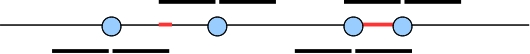
\includegraphics[scale=0.8]{over.jpg}
 \caption{Overestimating the Probability - Overlapping regions shown in Red}
 \label{fig:over}
\end{figure}

Now we consider regions with seperation of lenght $\frac{X_i}{2}$ we can easily see that since $\frac{X_i}{2} < X_i$ if the point is within this interval from the other points it will surely be part of the shortest segment. Since we are considering exactly half the distance there will be NO overlap, but we can see that there are regions which could actualy accomodate the point but is not considered by the algorithm, hence this is actually underestimating the probability. Substituting this in the above equation we get. 

\begin{eqnarray}
  Pr [ \varepsilon_{i+1} ] \geq 2i\frac{X_i}{2} = i X_i
\end{eqnarray}

Figure \ref{fig:under} will make things clear
\begin{figure}
 \centering
 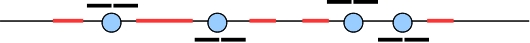
\includegraphics[scale=0.8]{under.jpg}
 \caption{Underestimating the Probability - Possible regions not considered shown in Red}
 \label{fig:under}
\end{figure}
Combining the two equation we get a range 

\begin{eqnarray}
i X_i \leq   Pr [ \varepsilon_{i+1} ] \leq  2iX_i
\end{eqnarray}

Substituting for $Pr [ \varepsilon_{i+1} ]$ in the equation we get 

\begin{eqnarray}
i X_i \leq  \frac{2}{i+1}  \leq  2iX_i
\end{eqnarray}

Since all numbers are positive hence taking multiplying throughout by $\frac{i}{X_i}$ and taking the inverse we get. 

\begin{eqnarray}
i^2 \leq  \frac{2i}{(i+1)X_i}  \leq  2i^2
\end{eqnarray}

Taking the inverse we have 

\begin{eqnarray}
\frac{1}{2 i^2} \leq  \frac{(i+1)X_i}{2i}  \leq  \frac{1}{i^2}
\end{eqnarray}

Since we need to find the asymptotic value we shall consider $i=n$, and we know $\frac{n+1}{n} \rightarrow 1$.

\begin{eqnarray}
\frac{1}{n^2} \leq {X_n}   \leq  \frac{2}{n^2}
\end{eqnarray}

Applying expectation we get. 

\begin{eqnarray}
\frac{1}{n^2} \leq {E[X_n]}   \leq  \frac{2}{n^2}
\end{eqnarray}

Since the other two are already free of any random variables. 

Hence not only are we able to prove that the expected length of the shortest segment $=O(n^2)$ but are able to prove a stronger result which says that the expected length of the shortest segment $=\Omega (n^2)$. 

\end{enumerate}




\end{answer}


\end{problem}
\pbitem
\begin{problem} 
\textbf{Smallest Enclosing Circle}\\
\begin{answer}
We will select a uniformly random sample $\frac{n}{2}$ out of the $n$  points given, let the set be $A$ and find the smallest possible circle $\mathbf{C}$ enclosing these points. Let us have set $S$ be the set of $n/2$ points that were not sampled. \\
Now for a single point $p_i$ in $S$ consider the set of points. $A \cup p_i$. 

We can see that if we find the probability of the point $p_i$ not being in the circle $C$, then we can easily expand it to the complete set $S$ as follows. 

Let us define the event $\varepsilon_i$ as the even that the point $p_i$ lies outside the circle. We also define the following random variable $X_i$ as follows 
\begin{equation}
  X_i = \left\{ 
  \begin{array}{l l}
    1 & \quad \text{if $p_i$ lies outside the circle}\\
    0 & \quad \text{otherwise}\\
  \end{array} \right.
\end{equation}

Now consider the enclosing circle for the set $A \cup p_i$, we can see that if $p_i$ lies outside the circle $\mathbf{C}$ then $p_i$ will be one of the points that define the new circle. We can now can preform a 
backward analysis on this point ($[\frac{n}{2} +1]^{th}$ ). The analysis is as
follows:\\

The point $p_i$ becomes part of the smallest enclosing circle $\mathbf{C}$ when it is one of the three points to form a  circle. Clearly the remaining two point must be from points within the $\mathbf{C}$ to extend $\mathbf{C}$ to include the new point.

Just like $A$ can be thought of as any random uniform set we can consider $A \cup p_i$ also as a random uniform set, since we will be considering all the $p_i$. Each combination fo $A \cup p_i$ is independent of the other $p_i$'s the $\mathbf{C}$ .

Now consider that there exists a enclosing circle for the set $A \cup p_i$. We can see that \\
\begin{equation}
 Pr[\text{$p_i$ outside the circle}] = Pr[\text{$p_i$ is one of the defining points of the circle}]
\end{equation}

Since each circle can have atmost $3$ defining point if we do a backward analysis we can see that 
 
\begin{equation}
Pr[\text{$p_i$ is one of the defining points of the circle}] \leq \frac{3}{\frac{n}{2} + 1}
\end{equation}
The $\leq$ comes from the fact that they circle may also have been defined with just two points. We shall now use this to find $E[X_i]$

\begin{equation}
E[X_i]  =   1 \cdot  Pr[\text{$p_i$ outside the circle}] + 0 \cdot (1- Pr[\text{$p_i$ outside the circle}])
\end{equation}

\begin{eqnarray}
E[X_i] & \leq \frac{3}{\frac{n}{2} + 1}
\end{eqnarray}

 We can see that $E[X]$ gives the expected number of points that will lie outside the circle. By linearity of expectation .

\begin{eqnarray}
X_i & = & \sum_{i=0}^{\frac{n}{2}}X_i \\
E[X_i] & = & \sum_{i=0}^{\frac{n}{2}}E[X_i] \\
& \leq & \sum_{i=0}^{\frac{n}{2}} \frac{3}{\frac{n}{2} + 1} \\
& \leq & 3 \cdot \frac{\frac{n}{2}}{\frac{n}{2} + 1}  \\
& \leq & 3
\end{eqnarray}
The answer is surprisingly a constant number, but in hindsight makes perfect sense.  

The expected number of unsampled points lie outside circle $\mathbf{C} < 3$
\end{answer}
\end{problem}

\pbitem 
\begin{problem} 
\textbf{Convex Hull problem}\\

\begin{enumerate}
\item \textbf{Backward analysis}\\
\begin{answer}
According to the algorithm discussed in class, each point is in some cone of the
data structure. Whenever a new point is taken for inserting 
inserting into the convex hull the cone gets split and thus the number of cone
change of point $p$ increases by one. It can be observed that
the expected running time of the algorithm is equivalent to the expected number of
cone changes caused by insertion of new point $p\in S$ to the Hull.

We know that the expectation of running time of the algorithm is $nlogn$. Let $X$
denote the total number of cone changes during the entire execution 
of the algorithm. Also $X_i$ denotes the number of cone changes for a point $p \in
S$. So we need to prove that 
\begin{equation}
Pr[Runnning \; Time > c nlogn] \leq \sum_{ p \in S} Pr(X_i > cE[X_i]) 
\end{equation}

It will be easier to take a microscopic view of the algorithm execution to find the
expected number of cone changes.Consider a point $p \in S$ which is to 
inserted into hull. Let $Y$ be a random variable that counts the number of cone
changes for the point $p$. Let $Y_i$ be a 0-1 random variable which 
indicates the contribution of $i^{th}$ iteration of algorithm to $Y$
\begin{equation}
E[Y_i ] = P r(There \; is \; a \; cone \; change \; for \; p).
\end{equation}

We will use backward analysis to find out the RHS of the above equation. The point
$p$ could have changed the cone if it was part of the cone created 
by the convex hull points $k$and $K+1$ during $(i-1)^{th}$ iteration and $k$
occurred during $i^{th}$ iteration. Thus the probability that $p$ had changed 
cone in $i^{th}$ iteration is equal to $\frac{2}{i}$. Thus\\

$E[Y_i]= \frac{2}{i}$

Which gives\\

$E[Y] = \sum_{1 \leq i \leq n} E[Z_i] $\\
  
= $\sum_{1 \leq i \leq n} \frac{2}{i}$\\

$E[Y]= H_n$\\

$E[Y]= ln \; n , since \; H_n = ln \; n $\\

$E[X_i]= ln \; n$\\

Now the expected number of cone changes can be obtained as follows.\\

$E[X]= \sum_{ p \in S} E[X_i]$\\

$E[X]= n * ln \; n$

Now we need to calculate $Pr [(X_i > cE[X_i])]$ which is same as $Pr(Y>cE[Y])$. As
$Y$ is sum of independent random variable we can apply 
Chernoff bound with $c = 1 + \delta $. \\

$Pr(X_i>cE[X_i]) \leq \Bigg(\frac{e^{c-1}}{c^c}\Bigg)^{E[X_i]}$\\

$\;\;\;\;\;\;\;\;\;\;\;\leq \Bigg(\frac{e^{c-1}}{e^{cln \; c}}\Bigg)^{E[X_i]}$\\

$\;\;\;\;\;\;\;\;\;\;\;\leq \Bigg(e^{-(cln \; c -c+1)} \Bigg)^{E[X_i]}$\\

$\;\;\;\;\;\;\;\;\;\;\;\leq e^{-(cln \; c -c+1)ln \; n}  $\\

$\;\;\;\;\;\;\;\;\;\;\;\leq n^{-(cln \; c -c+1)}$\\

From equation (2-1)\\

$Pr[Runnning \; Time > c nlogn] \leq \sum_{ p \in S} Pr(X_i > cE[X_i]) $

$\;\;\;\;\;\;\;\;\;\;\;\leq n * Pr(X_i > cE[X_i]) $\\

$\;\;\;\;\;\;\;\;\;\;\;\leq n * n^{-(cln \; c -c+1)}$\\

$\;\;\;\;\;\;\;\;\;\;\;\leq n^{-(cln \; c -c)}$\\
\end{answer}
\item \textbf{RQsort analysis method}\\
\begin{answer} 
\end{answer}
\end{enumerate}
\end{problem}


\pbitem
\begin{problem} 
\textbf{Analysing the duration of a randomized experiment by partitioning it into stages} \\
\begin{answer}

We shall look at a slight modification of the algorithm, and prove bounds on that can carried forward to the current algorithm, and then prove the bounds. \\
\textbf{Modified Algorithm}\\
\begin{enumerate}
 \item Initialise and set $E$ as all $\binom{n}{2}$ edges, and $V = \{ 1, \ldots n \}$.
\item Select the first edge randomly and add them to the set of connected components. 
\item Till graph is connected do the following. Select a edge uniformly randomly from the set $E$ without replacement, let it be $(u,v)$. 
\begin{enumerate}
 \item If it creates a cycle add the edge  
 \item Else discard the edge. (Point of difference with original algorithm)
\end{enumerate}
\end{enumerate}
Cycles in no way will help the connectedness of the graph hence keeping them will be of no use.  \\
Let $X_a$ be the running time of the actual algorithm and $X_m$ be the running time of the modified algorithm.\\

We can also see that since all $\binom{n}{2}$ edges exists, this method will ultimately reach a solution, and hence completion is also assured. \\

Now we shall partition the random experiment into different stages, let the $i^{th}$ stage be the stage where $|A| = i$ we can see that the first two stages are reached in time 1. Let us define the random variable $X_mi$ as the time spent in the $i^{th}$ step in the modified algorithm. Since once we leave each step we are not coming back to that (since we are only adding elements to $A$) we can see that. See that if we add $n-1$ edges and we have no cycles then we have to have a connected component. 

\begin{eqnarray}
 X_m = X_{m1}+ X_{m2} + \ldots + X_{mn}
\end{eqnarray}
What we need to find is the expected value of $X_m$, which we will denote by $E[X_m]$
Applying linearity of expectation we arrive at
\begin{eqnarray}
 E[X_m] = E[X_{m1}]+ E[X_{m2}] + \ldots + E[X_{mn}]
\end{eqnarray}

We already know the initial conditions that 

\begin{eqnarray}
 E[X_{m1}] = 0 \\
 E[X_{m2}] = 1 
\end{eqnarray}

Now consider the $i^{th}$ stage, we shall now consider the probability that it will move in a single step, let us look at the set of edges, out of the total $\binom{n}{2}$ edge the edges between the same components are not useful, considering that we have $i$ edges already added, let the size of a compenent be denoted by $C_i$
\begin{eqnarray}
i =  \sum_{\forall compenents \; j} C_j  
\end{eqnarray}
Considering this the total number of useless components $U$ in the set can be seen as 
\begin{eqnarray}
U =\frac{1}{2} \cdot \sum\sum_{\forall compenents \; (i,j)} (C_j)(C_i)
\end{eqnarray}
To maximise this we can set the number of compenent to be 1, and $C_1=i$. We are maximising the bad conditions  since we need the upperbound, in actual case it will be much less . 
We shall now look at the probability that an edge selected is useful . \\
This is nothing but seeing the probability of selecting a useful edge .
\begin{eqnarray}
Pr[Useful] & = & \frac{\binom{n}{2} - U}{\binom{n}{2} - \textrm{Edges selected till now}}\\
Pr[Useful] & \geq & \frac{\binom{n}{2} - \binom{i}{2}}{\binom{n}{2}} 
\end{eqnarray}
We can see that once we get even a single good event we will stop, hence we have been given a random experiment with $Success$ probability $p$ and we need to determine the expected number of trials until one success. This is given by $\frac{1}{p}$

\begin{eqnarray}
E[X_{i+1}] & \leq & \frac{\binom{n}{2}}{\binom{n}{2} - \binom{i}{2}} \\
 & \leq & \frac{n^2}{n^2 - i^2}
\end{eqnarray}

Summing this as shown in the formula we have. 

\begin{eqnarray}
E[X] & = & \sum_{i=1}{n-1}E[X_i] \\
& \leq & \sum_{i=1}{n-1} \frac{n^2}{n^2 - i^2} \\
& \leq & {n^2} \sum_{i=1}\frac{1}{(n+1)(n-1)} \\
& \leq & {n^2} \sum_{i=1}\frac{1}{2n} \left( \frac{1}{n+i} + \frac{1}{n-i} \right) \\
& \leq & \frac{n^2}{2n} \sum_{i=1}\frac{1}{2n} \left( \frac{1}{n+i} + \frac{1}{n-i} \right) \\
& \leq & \frac{n^2}{2n} (\frac{1}{1} + \frac{1}{2} + \ldots + \frac{1}{n-1} + \frac{1}{n} + \frac{1}{n+1} + \ldots \frac{1}{2n-1}) \\
& \leq & \frac{n}{2} H_{2n-1} \\
& \leq & \frac{n \; log 2n }{2}
\end{eqnarray}
This is the best possible bound that we are able to obtain. 
\end{answer} 
\end{problem}
\pbitem
\begin{problem}
\textbf{Online Sampling} \\
 \begin{answer}

We shall use the following algorithm to sample, let $S$ be the set of elements we are maintaining, and $U$ be the set of elements we are sampling from.  

\begin{algorithm}[H]                      % enter the algorithm environment
\caption{$OnlineSample(U)$}         	% give the algorithm a caption
\label{os}                           % and a label for \ref{} commands later in the document
\begin{algorithmic} 
\FOR{$i$ from $1\ldots n$}
 \STATE $S[i] \leftarrow U[i]$
\ENDFOR
\STATE Permute $S[i]$.
\FOR{$i$ from $n+1 \ldots m$}
 \STATE $RandVar \leftarrow rand(1, i+1)$
 \IF {$RandVar > n$ } 
   \STATE $Discard Apple$
 \ELSE
  \FOR {$j$ from $n \ldots RandVar$}
  \STATE $S[j] \leftarrow S[j-1]$
 \ENDFOR
 \STATE $S[RandVar] \leftarrow U[i]$
 \ENDIF
 \ENDFOR
 \STATE Return $S$
\end{algorithmic}
\end{algorithm}
\textbf{Explanation} \\
The algorithm does the following, it selects all the first $n$ elements. now for each new element coming after it consider the following situation.\\
Consider the apples as an ordering and then if we need to insert it, there are exactly $(n+1)$ position, to do it, and hence we insert it in one of the position and output the first $n$ apples.\\
For each apple we throw away we maintain a "ghost element" in our mind to find out the number of positions the next apple can be inserted into. , and do the same thing. \\
Since at each point of time, no apple moves backward, an apple discarded is permanent, and hence we need to maintain only the ghost of the apples discarded. \\

\begin{figure}[H]
 \centering
 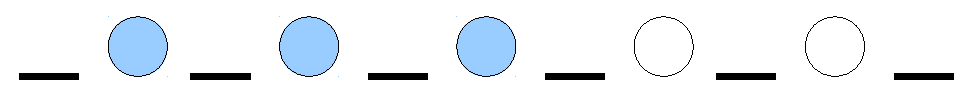
\includegraphics[scale=0.7]{os.eps}
 \caption{With n=3 inserting the 6th apple, the ghost apples which are already discarded are shown in white}
 \label{fig:os}
\end{figure}

\textbf{Proof of Correctness}
We give the following proofs for the correctness of the algorithm. The first thing we can see is f we consider all the permutation of the elements seen till then, then the first $n$ elements form exaclty what we desire, but the problem being it requires $m$ space now we will prove that the above algorithm achieves the same result with $n$ space. 
\begin{enumerate}
 \item \textbf{Informal proof using Backward Analysis} \\
 Since this is a online sampling experiment which cannot be backtracked, we can see that at each point of time we should have a selection that is the result of uniformly, randomly, independently selecting $n$ apples till then. T \\
\begin{figure}[H]
 \centering
 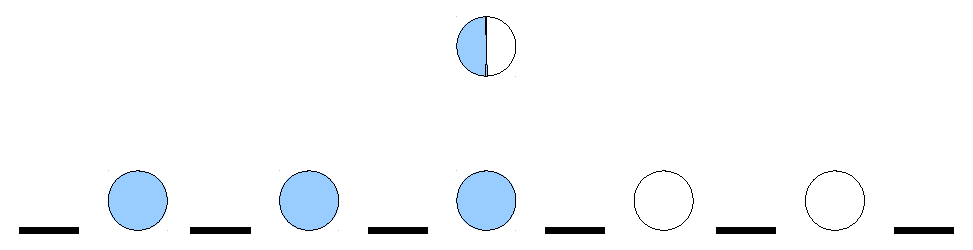
\includegraphics[scale=0.7]{osremove.eps}
 \caption{Given that there were 6 apples, and the 6 apple was removed where could it have been removed from}
 \label{fig:osremove}
\end{figure}
 Let the $i^{th}$ step be completed and the $i^{th}$ apple be either discarded (kept as ghost elements), or kept in the ordering, now consider the condition just before it is placed, given that it was placed in some location, there are exactly $i$ locations in which it can be placed, and since it is a uniform random distribution we can see that it should have been placed in any of the places with equal probability. Hence, our method of taking a random integer from $1$ to $i+1$ works, since we need to only consider if it is placed, we will only check if the number is $\leq n$. Now once we have placed the element it has to move the other elements appropriately. 
\item \textbf{Formal Proof using Induction} \\
 \begin{enumerate}
  \item It works for the trivial case $n$ apples since they are explicitly permuted. 
  \item Now assume that it works for the case where we have sampled $k$ apples. We have ordered and stored $n$ apples, since for the discarded apples order doesn't matter we just keep a count of the number.
\item Now consider the $k+1^{th}$ apple, we can see that if we already know that with the $k$ apples we already have the permutation, out of which the first $n$ apples are chosen, since we will never chosed the rest of the apples as said, we need to maintain only their count, and think as if they exists, then placing the apples as seen in the last image, will give a totally uniform distribution. Placing of the apples in the possible $(k+1)$ location is nothing but uniformly randomly placing them in the total ordering and checking if it is comes in the first $n$ elements or not. 
 \end{enumerate}


\end{enumerate}


 
 \end{answer}

\end{problem}

\end{problemlist}

\end{document}
